\documentclass{article}

\usepackage{xcolor}
\usepackage{tcolorbox}
\usepackage{awesomebox}
\usepackage{lastpage}
\usepackage{hyperref}
\usepackage{enumitem}
\usepackage{tabularx}
\usepackage{pdfpages}



\newcommand\gauchedroite[2]{\noindent{}#1\hfill#2}



%%%%%%% Définition des marges et bordure %%%%%%%%%
\usepackage[left=3cm,right=3cm,top=2cm,bottom=4cm]{geometry}



%%%%%%%% Pied de page %%%%%%%%%

\usepackage{fancyhdr}

\pagestyle{fancy}
\fancyhf{} % Efface les en-têtes et pieds de page précédemment définis

\rfoot{Page \thepage/\pageref{LastPage}}

\renewcommand{\headrulewidth}{0pt} % Ligne en haut de la page
\renewcommand{\footrulewidth}{0.4pt} % Ligne en bas de la page

%%%%%%%%%%%%%%%%%%%%%%%%%%




\begin{document}


\begin{tcolorbox}
    \gauchedroite{PFA - 2023/2024}{ENSEIRB MATMECA}
    
    \begin{center}
        \fontsize{17pt}{15pt}\selectfont
            \textbf{\color{black}Cahier des Charges - EcoScout}
        \selectfont
    \end{center}
\end{tcolorbox}


\begin{figure}[b]
    \begin{center}
        
\includegraphics[width=5cm]{pictures/logoEnseirbMatmeca.jpg}
    \end{center}
\end{figure}

\newpage

\tableofcontents

\vspace{20px}

\section*{Membres de l'équipe}

\begin{table}[htbp]
    \centering
    \begin{tabular}{|l|l|l|p{4cm}|}
        \hline
        \textbf{Prenom} & \textbf{Nom} & \textbf{Rôle pour ce projet} \\
        \hline
        Amira & Elouazzani & Développeuse \\
        \hline
        Arthur & Durand & Développeur \\
        \hline
        Arthur & Hermitte & Développeur \\
        \hline
        Chloé & Le Maitre & Développeuse \\
        \hline
        Malek & Mkadem & Développeuse \\
        \hline
        Théophane & Loloum & Développeur \\
        \hline
        Thomas & Tuilier & Développeur \\
        \hline
        Sam & Gubernator & Développeur \\
        \hline
        Sylvain & Lombardy & Enseignant ENSEIRB, responsable du projet \\
        \hline
        Matthieu & Ploquin & Client du projet - Groupe SGdF Orée de Brocéliande \\
        \hline
        Gabriel & & Utilisateur - Chef bleu SGdF, groupe de Pacé (35) \\
        \hline
        Stéphane & & Utilisateur - Responsable de groupe SGdF, groupe de La Ferté St Aubin (45) \\
        \hline
    \end{tabular}
\end{table}

\newpage

%%%%%%%%%%%%%%%%%%%%%%%%%%


\section{Présentation du projet}
\subsection{Introduction}
Ce projet est un projet réalisé dans le cadre d'un PFA (Projets au fil de l'année)
de l'école ENSEIRB-MATMECA de Talence durant l'année scolaire 2023/2024. \\
\newline
Il vise à développer une application informatique permettant d’inciter chaque adhérent
et chaque structure à limiter son impact sur le climat, notamment en mesurant les 
progrès réalisés au travers de différentes actions. L'application sera élaborée en prenant en compte l'expérience et les besoins spécifiques des Scouts et Guides de France. Toutefois, sa conception la rendra accessible à toute structure souhaitant s'engager dans une démarche similaire en faveur de la réduction de son empreinte écologique. L'application sera accessible via une interface web conviviale, facilitant ainsi l'utilisation sur divers appareils. 
\\
\newline
Le projet EcoScout est disponible sur GitHub, accessible à l'adresse suivante :
\begin{center}
    \url{https://github.com/tloloum/EcoScout}
\end{center}
Le code source du projet EcoScout est publié en tant que logiciel open source, 
ce qui signifie que le code est librement accessible et modifiable par la communauté. 


\subsection{Définition des termes du projet}

Différents termes importants seront utilisés lors de la réalisation de ce projet, en voici une liste non exhaustive.
\begin{itemize}
    \item \textbf{Utilisateur} : Une personne qui utilise l'application
    \item \textbf{Structure} : Un utilisateur moral utilisant l'application
    \item \textbf{Responsable:} Utilisateur responsable d'une structure donnée.
    \item \textbf{Événement:} Événement planifié avec une durée définie organisé par une structure.
    \item \textbf{Défi:} Jeu invitant des structures à atteindre un ou plusieurs objectifs dans un temps donné (qui peut être lié à un événement ou une structure ou un utilisateur).
    \item \textbf{Objectif:} Défini par une mesure (un élément qui peut se mesurer), une valeur (une donnée chiffrée ou référence) 
    et un critère (un opérateur de comparaison). 
\end{itemize}

Les \textbf{Défis} dans l'application EcoScout sont définis comme un ensemble d' \textbf{Objectifs} 
à atteindre dans un temps donné, avec des critères spécifiques. La \textbf{base d'objectifs} 
fournie dans l'application sert de point de départ, offrant une variété d'objectifs aux utilisateurs. 
Chaque \textbf{structure} a la capacité de créer ses propres objectifs. Les objectifs créés par une 
structure sont visibles par toutes les structures qui en dépendent, favorisant la transparence et la collaboration. 

\begin{tcolorbox}[colback=white!2,
    colframe=black!60,
    title=\textbf{Exemple de Défis}
   ]
   Le \textbf{Groupe de Chamarande} crée un défi appelé "Déplacements Carbonés" dont les objectifs spécifiques peuvent inclure la réduction des émissions de carbone 
   liées aux déplacements. Les structures dépendantes, comme \textbf{L'Unité Louveteaux-Jeannettes}, 
   participent activement à la réalisation de ces objectifs.
\end{tcolorbox}


\begin{tcolorbox}[colback=white!2,
    colframe=black!60,
    title=\textbf{Exemple d'utilisation}
   ]
   \textbf{Yanis Toirscout} est un utilisateur d'EcoScout. Il utilise l'application 
    pour gérer et suivre les activités de son groupe de Chamarande.\\
    \newline
    \textbf{Groupe Chamarande} représente la structure regroupant différentes 
    unités et membres. Ici \textbf{Yanis Toirscout} est le responsable du \textbf{Groupe Chamarande}.
    \textbf{L'unité Louveteaux-Jeannettes} est membre du \textbf{Groupe Chamarande}. 
    Par exemple on pourrait avoir Alice, fille de Yanis, qui fait partie de l'unité Louveteaux-Jeannettes.\\
    \newline
    Le \textbf{Week-end Déplacements Durables} peut être un événement organisé par le \textbf{Groupe Chamarande}.
    Il sera définie dans un délai prédéterminé, ici un weekend. Le \textbf{Défi} de cet événement pourrait être 
    d'inviter les différentes structures spécifique à limiter leur empreinte carbone a un certain nombre.
\end{tcolorbox}

\begin{figure}[h]
    \centering
    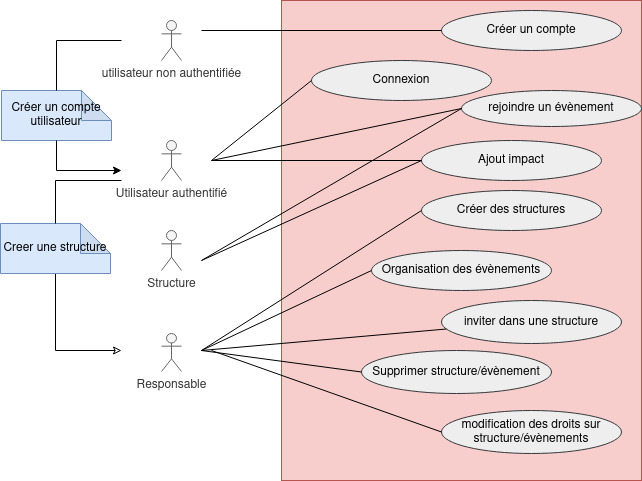
\includegraphics[width=0.8\linewidth]{pictures/use_case_pfa.jpg}
    \caption{Diagramme de cas d'utilisation}
    \label{fig:diag_use_case}
\end{figure}




\subsection{Règles définies}
Différentes règles ont été définies par rapport à l'interaction des différents éléments du projet.
\begin{itemize}
    \item Une structure a entre 1 et n responsables.
    \item Un utilisateur est responsable de sa structure "personne physique".
    \item Un utilisateur peut être responsable de 1 à n structures.
\end{itemize}

\begin{figure}
    \centering
    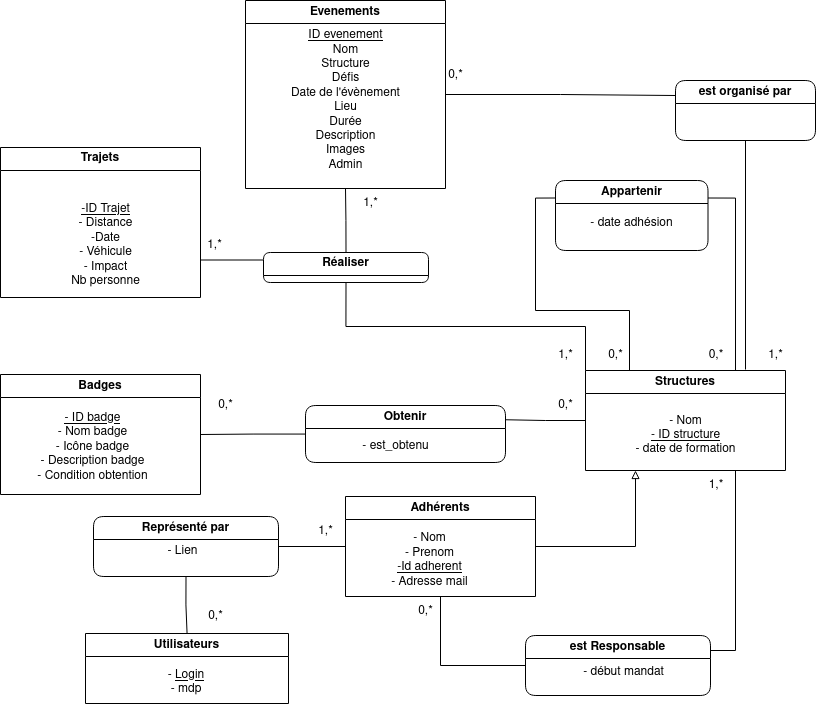
\includegraphics[width=1.1\linewidth]{pictures/diag_concept.png}
    \caption{Diagramme conceptuel}
    \label{fig:diag_concept}
\end{figure}



\newpage

\newgeometry{left=2cm, right=2cm, top=2cm, bottom=2cm}
\section{Spécifications Fonctionnelles Détaillées}
\subsection{Spécifications Indispensables}

\begin{itemize}
    \item \textbf{Créer un compte :} Définir un utilisateur avec ses informations primordiales (login, nom, prénom, mail, numéro d'adhérent)
    \item \textbf{Créer une structure :} Capacité d'un utilisateur de créer une structure. Celui-ci devient responsable et aura alors les droits de modifications de la structure lui permettant de : 
    \begin{itemize}
        \item Rajouter/Supprimer des informations à renseigner pour rejoindre cette structure
        \item Créer des utilisateurs dans cette structure avec des informations de bases(en attendant que les personnes rejoignent la structure avec leurs propres comptes).
        \item Faire rejoindre sa structure à une autre (hiérarchie des structures)
        \item Inviter un utilisateur à rejoindre sa structure via un lien d'invitation. 
    \end{itemize}
    \item \textbf{Ajout d'une action ayant un impact écologique} : Capacité d'un utilisateur/d'une structure de rajouter un impact écologique (exemple : un trajet en voiture)
\end{itemize}

\subsection{Spécifications Importantes}

Étant donné que le terme 'important' peut prêter à confusion en raison de sa nature vague, les spécifications qualifiées d'importantes sont clairement hiérarchisées et triées par ordre de priorité pour garantir une compréhension et une mise en œuvre précises de ces éléments clés du projet

\begin{itemize}
    \item \textbf{1. Organiser un événement :} Un utilisateur ou le responsable d'une structure à la capacité de définir un événement sur une durée fixe et de rajouter/inviter des utilisateurs/structures dans cet événement. Un événement peut contenir plusieurs événements (ex : une année est considérée comme un événement durant laquelle les week-ends sont aussi des événements).
    \item \textbf{2. Suppression d'une structure ou d'un événement :} Capacité d'un responsable à supprimer un événement ou une structure crée.
    \item \textbf{3. Partage des droits sur une structure :} Un responsable peut partager les droits de modification d'une structure avec d'autres utilisateurs
    \item \textbf{4. Affichage de statistiques globales :} Calcul et affichage de statistiques sur son impact écologique d'une structure ou d'un événement (moyenne, progression/comparaison des impacts sur une durée). 
\end{itemize}

\subsection{Spécifications Secondaires}
\begin{itemize}
    \item \textbf{Ajout d'objectifs :} Un responsable peut rajouter des objectifs pour sa structure ou son événement.
    \item \textbf{Ajout défis :} Un responsable peut regrouper un ensemble d'objectifs à atteindre sur un temps donnée (par exemple lors d'un événement). 
    \item \textbf{Attribution de récompense à la réalisation de défis :} L'accomplissement de défis peut amener à la récupération de récompense, comme un badge, attribué à un utilisateur. 
\end{itemize}

% \begin{table}[h]
% \centering
% \begin{tabularx}{\textwidth}{|X|X|X|X|X|}
%     \hline
%     \textbf{Fonctionnalité} & \textbf{Description} & \textbf{Complexité} & \textbf{Priorité} & \textbf{Justification} \\
%     \hline
%     \textbf{Créer un compte} & Définir un utilisateur (nom, prénom, ... ) & Simple & \textit{Indispensable} & Création de BDD \\
%     \hline
%     \textbf{Faire des groupes} & Rejoindre plusieurs utilisateurs, avec un/des administrateur(s) qui a le droit de modification (suppression de données non valables) & Simple & \textit{Indispensable} & BDD \\
%     \hline
%     \textbf{Organisation d'événements} & Définir un événement sur une durée fixe et rajouter des utilisateurs/groupes dans cet événement & Moyen & \textit{Important} & \\
%     \hline
%     \textbf{Lien d'invitation dans un groupe} & Permettre à un administrateur d'inviter des utilisateurs dans un groupe & Moyen & \textit{Indispensable} & \\
%     \hline
%     \textbf{Définir un événement public / privé} & Permettre à des personnes de s'ajouter sans invitation à un événement/groupe & Moyen & \textit{Secondaire, à proposer} & \\
%     \hline
%     \textbf{Calcul de l'impact} & Calculer l'impact écologique d'un groupe/d'une personne/d'un événement. Sur un temps choisi/une action particulière (ex: le trajet) & Difficile & \textit{Important} & \\
%     \hline
%     \textbf{Ajout d'un impact écologique} & Un utilisateur/un groupe peut rajouter des actions qui ont un impact écologique & Moyen & \textit{Indispensable} & \\
%     \hline
% \end{tabularx}
% \end{table}

% \newpage 

% \begin{table}[h]
%     \centering
%     \begin{tabularx}{\textwidth}{|X|X|X|X|X|}
%     \hline
%     \textbf{Rechercher une action qui a un impact écologique} & Rechercher une action pour la rajouter dans les impacts d'un utilisateur / groupe / événements & Simple/Moyen & \textit{Important} & Utilisation de la BDD de l'ADEM \\
%     \hline
%     \textbf{Côté ludique (badge,...)} & Rajout d'un côté ludique à l'application, et ne pas donner un aspect de compétition & Difficile & \textit{Secondaire} & Ensemble de fonctionnalités secondaires, complexité difficile à calculer \\
%     \hline
%     \textbf{Statistiques globales (progression sur le temps, impacts des actions)} & Calcul des statistiques globales d'un groupe/événements. (moyennes, comparaison sur le temps,...) & Moyen & \textit{Important} & \\
%     \hline
%     \textbf{Suppression d'un groupe / événements} & Capacité de pouvoir supprimer un groupe/événements par un administrateur de celui-ci & Facile & \textit{Important} & \\
%     \hline
%     \textbf{Suppression automatique (événements / groupes trop anciens / passés)} & Suppression automatique des événements ou des groupes dont l'activité est inexistante depuis trop longtemps & Moyen & \textit{Secondaire} & \\
%     \hline
%     \textbf{Ajout de droits sur un groupe} & L'administrateur initial d'un groupe ou d'un événement peut rajouter des droits à certains utilisateurs sur ce groupe & Facile &  & \\
%     \hline
% \end{tabularx}
% \end{table}

\newpage 

\restoregeometry

\section{Pages de l'application}

Chaque fonctionnalité clé sera représentée par une page dédiée dans l'application pour assurer une navigation intuitive. Voici comment les différentes fonctionnalités seront intégrées en tant que pages de l'application :

\begin{itemize}[label=-]
    \item \textbf{Page d'Accueil (Dashboard) :} Cette page constituera le point central de l'application, permettant aux utilisateurs de gérer leur compte, afficher un résumé personnalisé de leurs activités, et accéder rapidement aux fonctionnalités principales.

    \item \textbf{Page des Utilisateurs (Profil) :} Les utilisateurs auront une page dédiée pour créer et gérer leurs comptes. Ils pourront également consulter leurs informations personnelles et préférences liées à l'application.

    \item \textbf{Page des Statistiques (Calcul d'Impact) :} Les statistiques globales concernant les événements, les structures, et les individus seront disponibles sur cette page. Les moyennes, les comparaisons sur le temps, et d'autres indicateurs écologiques seront présentés de manière claire. Cette page offrira aux utilisateurs la possibilité de visualiser l'impact écologique de leurs actions, de leurs dépenses carbones, avec une distinction entre les dépenses communes et individuelles.. Le calcul d'impact sera alimenté par la base de données de l'ADEME. 

    \item \textbf{Page des Structures :} La création et la gestion de structures seront accessibles depuis cette page. Les utilisateurs pourront inviter d'autres membres, définir des relations entre eux, et créer des structures de différentes tailles.

    \item \textbf{Page des Badges :} Bien que secondaire, la page des badges présentera le côté ludique de l'application, récompensant les utilisateurs pour leurs actions écologiques.

    \item \textbf{Page d'Organisation d'Événements :} Les utilisateurs pourront organiser des événements, tels que des week-ends de groupe, directement depuis cette page.

\end{itemize}
Nous allons maintenant voir le parcours que pourra faire un utilisateur sur l'application. \\
\newline
\textbf{Etape 1 - Connexion - Page d'accueil}\\
Sur la page d'accueil, un \textit{utilisateur} peut se connecter via son \textit{login}. Si ce dernier n'appartient pas encore à la base de données. Il peut rentrer les différentes informations (Nom / Prenom / Adresse mail / Login) pour pouvoir créer son compte. \\
\newline 
La protection de la connexion sera réalisée avec un mot de passe ou alors un système de code à rentré envoyé à l'utilisateur. \\
\newline
\textbf{Etape 2 - Créer une structure - Page des structures}\\
Une fois connecté, l'utilisateur souhaite créer son équipe \textit{L’Unité Louveteaux-Jeannettes} et rejoindre via cette équipe le \textit{Groupe de Chamarande}.\\
\newline
La première étape est donc de créer \textit{L’Unité Louveteaux-Jeannettes} et de la partager aux membres. L'utilisateur se rend donc dans le menu structures et \textit{Créer une structure}. Il va devoir rentrer le nom de la structure, une description et, de façon optionnelle la date qui représente la date de création de la structure. Si cette date n'est pas spécifiée, la date de création sera automatiquement définie comme la date à laquelle la structure a été créée dans l'application. L'utilisateur qui a crée cette structure est considéré comme un responsable de cette structure.\\
\newline
Une fois la structure créé, elle devrait être visible dans la liste des structures. Si on la sélectionne on peut voir les informations de la structure comme le nombre de membres par exemple. \textit{L’Unité Louveteaux-Jeannettes} ne possède ici qu'un seul membre qui est l'utilisateur qui a créé cette structure. Il peut, car il est un responsable de la structure, inviter des nouveaux membres, trouvables via login ou mail. Si d'autres membres rejoignent la structure, les utilisateurs qui sont responsables de la structure peuvent élire d'autres responsables en plus.\\
\newline
\textbf{Etape 3 - Rejoindre une structure - Page des structures}\\
Deux situations sont possibles pour rejoindre une structure. 
\begin{itemize}
    \item Si on a reçu une invitation (par notification ou par mail), on peut accepter l'invitation et rejoindre la structure (même situation pour un événement). Si la personne qui souhaite rejoindre n'a pas encore de compte (donc forcément dans une situation où l'invitation a été reçue par l'autre). 
    \item Si un utilisateur décide de rejoindre une structure directement. Pour réaliser cela, il suffit de se rendre sur la page de la structure et de cliquer sur rejoindre. A partir de ce moment-là, un menu lui demandera s'il souhaite rejoindre en tant que personne ou rejoindre via une structure dont il est responsable (il sera donc possible d'en sélectionner un). Il est donc possible d'appartenir directement ou indirectement à une structure. L'invitation devra donc être accepté par un responsable.
\end{itemize}
\textbf{Remarque :} Dans le cas ou l'on souhaite donnée les droits de responsables à une "sous-structure" qui appartient à notre structure, alors seulement les responsables de cette "sous-structure" seront responsable de la structure.\\
\newline 
\textbf{Etape 4 - Evènement}\\
De la même manière que pour les structures, il est possible de créer et de rejoindre un événement. Un événement est défini par une date de début, une date de fin, une description et, si l'on souhaite, des défis. \\
\newline 
\textbf{Etape 5 - Impact}\\
Il est possible, pour un événement de rajouter des actions qui ont un impact écologique. Lorsqu'un utilisateur ajoute une action, il l'ajoute dans un événement. Cependant, cette action est reliée à l'utilisateur, elle sera donc visible dans cet événement, mais aussi sur le profil de l'utilisateur et dans les structures où l'utilisateur est présent si ses structures appartiennent à cet événement. 





\newpage
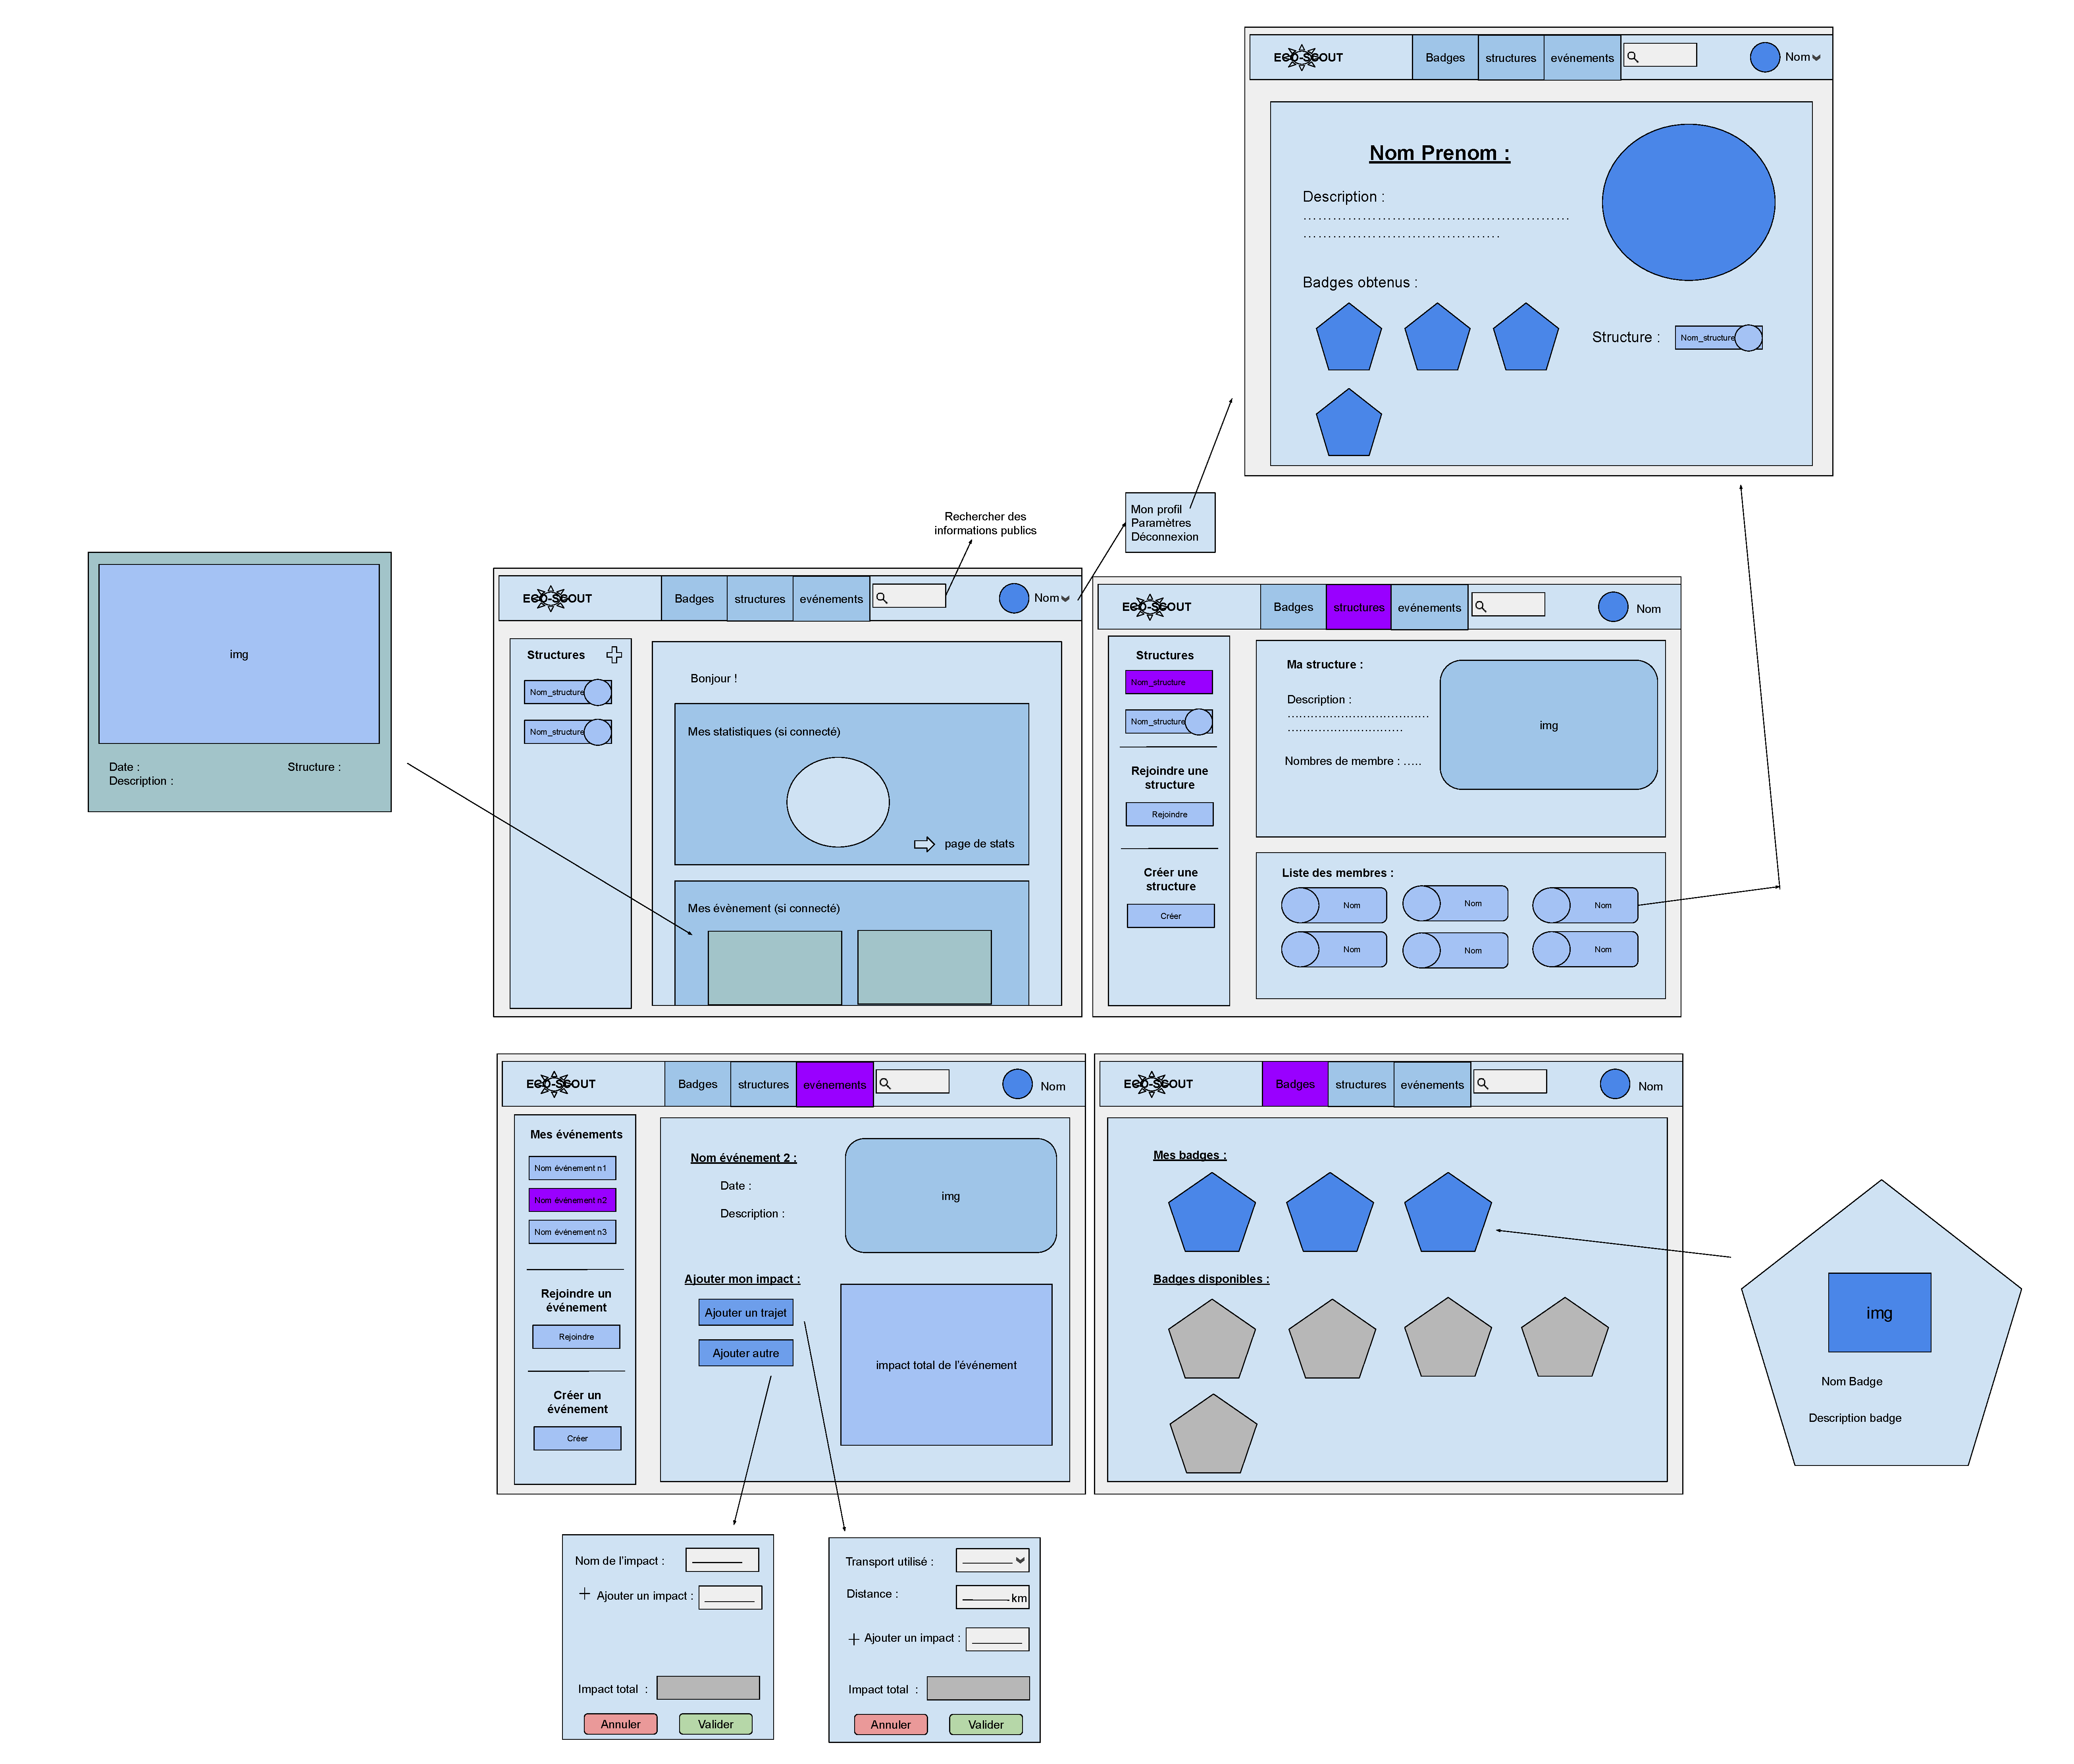
\includepdf{./pictures/vues_app.pdf}

\end{document}